\documentclass{standalone}
\usepackage[utf8]{inputenc}
\usepackage{amsmath}
\usepackage{amsfonts}
\usepackage{amssymb}
\usepackage{tikz}
\usetikzlibrary{calc}

% GanttHeader setups some parameters for the rest of the diagram
% #1 Width of the diagram
% #2 Width of the space reserved for task numbers
% #3 Width of the space reserved for task names
% #4 Number of months in the diagram
% In addition to these parameters, the layout of the diagram is influenced
% by keys defined below, such as y, which changes the vertical scale
\def\GanttHeader#1#2#3#4{%
 \pgfmathparse{(#1-#2-#3)/(#4)}
 \tikzset{y=7mm, task number/.style={left, font=\bfseries},
     task description/.style={text width=#3,  right, draw=none,
           font=\sffamily, xshift=#2,
           minimum height=2em},
     gantt bar/.style={draw=black, fill=blue!30},
     help lines/.style={draw=black!30, dashed},
     x=\pgfmathresult pt
     }
  \def\totalmonths{#4}
  \node (Header) [task description] at (0,0) {\textbf{\large }};
  \begin{scope}[shift=($(Header.south east)$)]
    \foreach \x in {1,...,#4}
      \node[above,rotate=90] at (\x,1) {\tiny\x};
 \end{scope}
}

% This macro adds a task to the diagram
% #1 Number of the task
% #2 Task's name
% #3 Starting date of the task (month's number, can be non-integer)
% #4 Task's duration in months (can be non-integer)
\def\Task#1#2{%
%\node[task number] at ($(Header.west) + (0, -#1)$) {#1};
\node[task description] at (0,-#1) {#2};
\begin{scope}[shift=($(Header.south east)$)]
  \draw (0,-#1) rectangle +(\totalmonths, 1);
  \foreach \x in {1,...,\totalmonths}
    \draw[help lines] (\x,-#1) -- +(0,1);
\end{scope}
}

% This macro adds a task to the diagram
% #1 Number of the task
% #2 Task's name
% #3 Starting date of the task (month's number, can be non-integer)
% #4 Task's duration in months (can be non-integer)
\def\TaskActive#1#2#3{%
\begin{scope}[shift=($(Header.south east)$)]
  \filldraw[gantt bar] ($(#2, -#1+0.2)$) rectangle +(#3,0.6);
\end{scope}
}

\begin{document}

\begin{tabular}{lr}
Scheduler: & RR-2 scheduler
\\
Input: & input/testdata3.txt
\\
Total Process Count: & 17
\\
Total Waiting Time: & 2094
\\
Average Waiting Time: & 123.17647
\\
Total Turnaround Time: & 2298
\\
Average Turnaround Time: & 135.17647
\\
Total Context Switch Count: & 106
\\
\end{tabular}
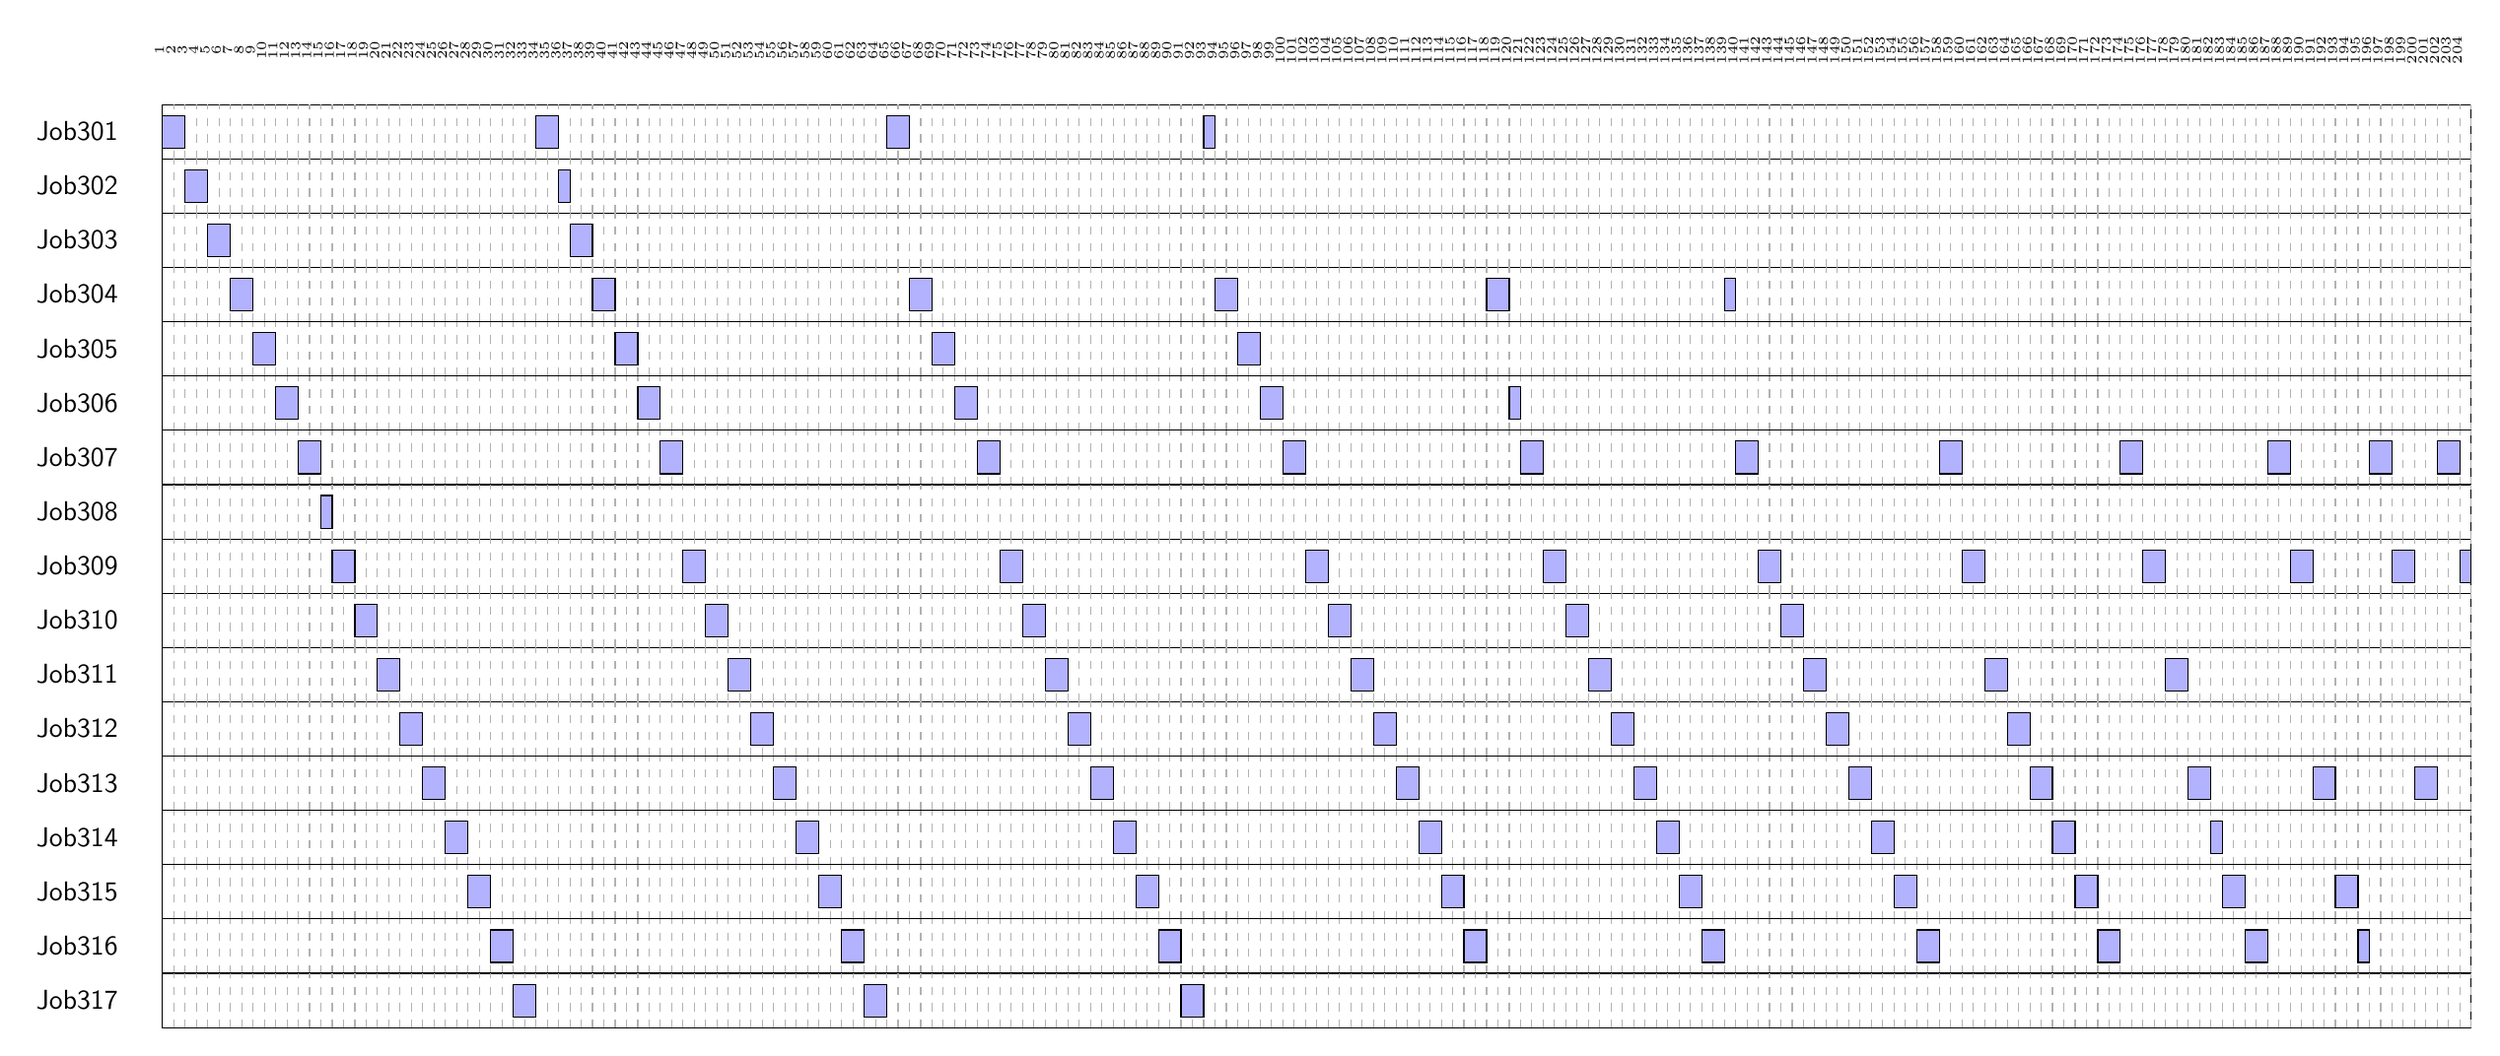
\begin{tikzpicture}
\GanttHeader{32cm}{5ex}{1.5cm}{204}
\Task{1}{Job301}
\Task{2}{Job302}
\Task{3}{Job303}
\Task{4}{Job304}
\Task{5}{Job305}
\Task{6}{Job306}
\Task{7}{Job307}
\Task{8}{Job308}
\Task{9}{Job309}
\Task{10}{Job310}
\Task{11}{Job311}
\Task{12}{Job312}
\Task{13}{Job313}
\Task{14}{Job314}
\Task{15}{Job315}
\Task{16}{Job316}
\Task{17}{Job317}
\TaskActive{1}{0}{2}
\TaskActive{2}{2}{2}
\TaskActive{3}{4}{2}
\TaskActive{4}{6}{2}
\TaskActive{5}{8}{2}
\TaskActive{6}{10}{2}
\TaskActive{7}{12}{2}
\TaskActive{8}{14}{1}
\TaskActive{9}{15}{2}
\TaskActive{10}{17}{2}
\TaskActive{11}{19}{2}
\TaskActive{12}{21}{2}
\TaskActive{13}{23}{2}
\TaskActive{14}{25}{2}
\TaskActive{15}{27}{2}
\TaskActive{16}{29}{2}
\TaskActive{17}{31}{2}
\TaskActive{1}{33}{2}
\TaskActive{2}{35}{1}
\TaskActive{3}{36}{2}
\TaskActive{4}{38}{2}
\TaskActive{5}{40}{2}
\TaskActive{6}{42}{2}
\TaskActive{7}{44}{2}
\TaskActive{9}{46}{2}
\TaskActive{10}{48}{2}
\TaskActive{11}{50}{2}
\TaskActive{12}{52}{2}
\TaskActive{13}{54}{2}
\TaskActive{14}{56}{2}
\TaskActive{15}{58}{2}
\TaskActive{16}{60}{2}
\TaskActive{17}{62}{2}
\TaskActive{1}{64}{2}
\TaskActive{4}{66}{2}
\TaskActive{5}{68}{2}
\TaskActive{6}{70}{2}
\TaskActive{7}{72}{2}
\TaskActive{9}{74}{2}
\TaskActive{10}{76}{2}
\TaskActive{11}{78}{2}
\TaskActive{12}{80}{2}
\TaskActive{13}{82}{2}
\TaskActive{14}{84}{2}
\TaskActive{15}{86}{2}
\TaskActive{16}{88}{2}
\TaskActive{17}{90}{2}
\TaskActive{1}{92}{1}
\TaskActive{4}{93}{2}
\TaskActive{5}{95}{2}
\TaskActive{6}{97}{2}
\TaskActive{7}{99}{2}
\TaskActive{9}{101}{2}
\TaskActive{10}{103}{2}
\TaskActive{11}{105}{2}
\TaskActive{12}{107}{2}
\TaskActive{13}{109}{2}
\TaskActive{14}{111}{2}
\TaskActive{15}{113}{2}
\TaskActive{16}{115}{2}
\TaskActive{4}{117}{2}
\TaskActive{6}{119}{1}
\TaskActive{7}{120}{2}
\TaskActive{9}{122}{2}
\TaskActive{10}{124}{2}
\TaskActive{11}{126}{2}
\TaskActive{12}{128}{2}
\TaskActive{13}{130}{2}
\TaskActive{14}{132}{2}
\TaskActive{15}{134}{2}
\TaskActive{16}{136}{2}
\TaskActive{4}{138}{1}
\TaskActive{7}{139}{2}
\TaskActive{9}{141}{2}
\TaskActive{10}{143}{2}
\TaskActive{11}{145}{2}
\TaskActive{12}{147}{2}
\TaskActive{13}{149}{2}
\TaskActive{14}{151}{2}
\TaskActive{15}{153}{2}
\TaskActive{16}{155}{2}
\TaskActive{7}{157}{2}
\TaskActive{9}{159}{2}
\TaskActive{11}{161}{2}
\TaskActive{12}{163}{2}
\TaskActive{13}{165}{2}
\TaskActive{14}{167}{2}
\TaskActive{15}{169}{2}
\TaskActive{16}{171}{2}
\TaskActive{7}{173}{2}
\TaskActive{9}{175}{2}
\TaskActive{11}{177}{2}
\TaskActive{13}{179}{2}
\TaskActive{14}{181}{1}
\TaskActive{15}{182}{2}
\TaskActive{16}{184}{2}
\TaskActive{7}{186}{2}
\TaskActive{9}{188}{2}
\TaskActive{13}{190}{2}
\TaskActive{15}{192}{2}
\TaskActive{16}{194}{1}
\TaskActive{7}{195}{2}
\TaskActive{9}{197}{2}
\TaskActive{13}{199}{2}
\TaskActive{7}{201}{2}
\TaskActive{9}{203}{1}
\end{tikzpicture}
\end{document}
